%!TEX root = main.tex
\section{Gesture Recognition}

\begin{frame}
\frametitle{What is a gesture?}

\begin{itemize}
\item A continuous stream of poses
\item The transfer of a subset of joints from point A to B, using a vaguely predefined trajectory
\end{itemize}
\end{frame}

\begin{frame}
\frametitle{What is a gesture?}
\begin{itemize}
\item \st{A continuous stream of poses}
\item \textbf{The transfer of a subset of joints from point A to B, using a vaguely predefined trajectory}
\end{itemize}

\end{frame}

\begin{frame}
\frametitle{Gesture Example}

\begin{center}
Swipe In (Right Hand)

\begin{figure}[!htb]
\centering
\resizebox{\linewidth}{!}{
	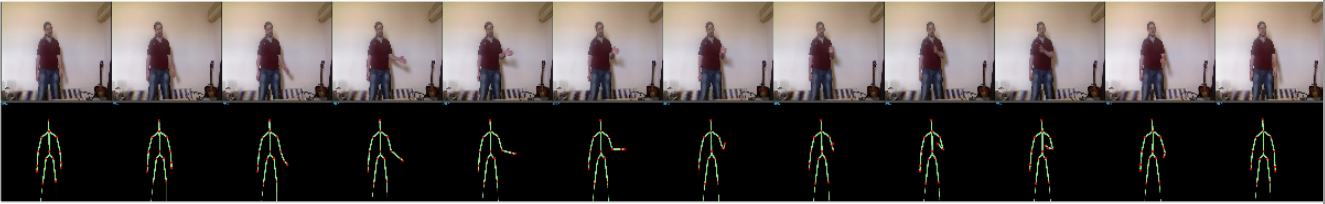
\includegraphics[]{figs/swipein-frameseq}
}
\end{figure}


\end{center}

\begin{center}
Swipe Up (Right Hand)

\begin{figure}[!htb]
\centering
\resizebox{\linewidth}{!}{
	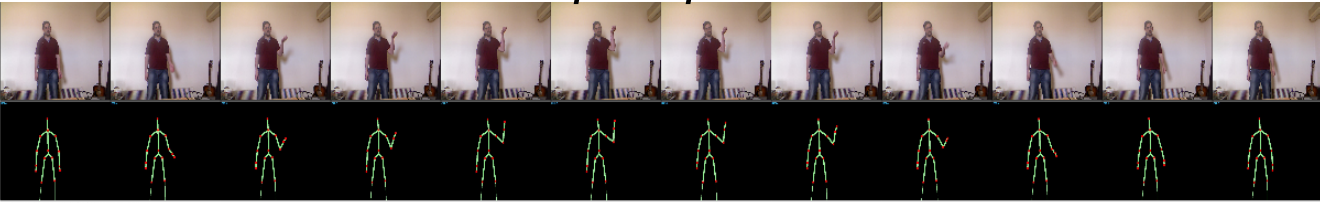
\includegraphics[]{figs/swipeup-frameseq}
}
\end{figure}


\end{center}
\end{frame}



\begin{frame}
\frametitle{The proposed approach}

\begin{itemize}
\item Extract a set of \textbf{low level geometric} features
\item Evaluate the performance (classification \textbf{accuracy} and \textbf{time}) of a set of well known machine learning techniques on this set of features
\end{itemize}

\end{frame}

\subsection{Feature Extraction}

\begin{frame}
\frametitle{Feature Extraction}

\begin{itemize}
\item We are interested in gestures; use only elbows, wrists and hands (LeftElbow, RightElbow, LeftWrist, RightWrist, LeftHand, RightHand)
\item For each we calculate a set of features, for the set of N frames that correspond to the gesture and based on their 3D coordinates
\end{itemize}

\end{frame}

\begin{frame}
\frametitle{Feature Properties}

Our features satisfy the following

\begin{itemize}
\item They require constant time \textbf{O(1)} in each frame to compute
\item Small gesture changes are reflected to small feature changes (angle and displacement are able to \textbf{discriminate between small movements})
\item They are aggregate features that \textbf{summarize} the gesture over all the frames
\item They are \textbf{small in size} (a feature vector in minified JSON format is about 3KB)
\end{itemize}

\end{frame}

\begin{frame}
\frametitle{The Features}

\begin{columns}[T]

\begin{column}{.4\linewidth}
Features are extracted
\begin{itemize}
\item from each skeletal \textbf{joint}
\item from a set of the \textbf{frames} depicting the gesture
\item using the \textbf{3D coordinates} of the joints
\end{itemize}

\end{column}

\pause

\begin{column}{.7\linewidth}
\resizebox{\linewidth}{!}{

    \begin{tabular}{|c|c|c|}
        \hline
         \textbf{Feature name}  & \textbf{Frames involved}  & \textbf{Equation}  \\ \hline
         Spatial angle          & $F_2, F_1$                  & $\displaystyle \frac{\mathbf{v}^{(J)}_{2} - \mathbf{v}^{(J)}_{1}}{\left\lVert \mathbf{v}^{(J)}_{2} - \mathbf{v}^{(J)}_{1} \right\rVert}$\\ \hline
         Spatial angle          & $F_n, F_{n-1}$              & $\displaystyle \frac{\mathbf{v}^{(J)}_{n} - \mathbf{v}^{(J)}_{n-1}}{\left\lVert \mathbf{v}^{(J)}_{n} - \mathbf{v}^{(J)}_{n-1} \right\rVert}$\\ \hline
         Spatial angle          & $F_n, F_{1}$              & $\displaystyle \frac{\mathbf{v}^{(J)}_{n} - \mathbf{v}^{(J)}_{1}}{\left\lVert \mathbf{v}^{(J)}_{n} - \mathbf{v}^{(J)}_{1} \right\rVert}$\\ \hline
         Total vector angle     & $F_1,\ldots, F_n$         & $\displaystyle \sum_{i=1}^n\arccos \left(\frac{\mathbf{v}^{(J)}_{i} \cdot \mathbf{v}^{(J)}_{i-1}}{\left\lVert \mathbf{v}^{(J)}_{i} \right\rVert \left\lVert \mathbf{v}^{(J)}_{i-1} \right\rVert}\right)$ \\ \hline
         Squared total vector angle     & $F_1,\ldots, F_n$         & $\displaystyle \sum_{i=1}^n\arccos \left(\frac{\mathbf{v}^{(J)}_{i} \cdot \mathbf{v}^{(J)}_{i-1}}{\left\lVert \mathbf{v}^{(J)}_{i} \right\rVert \left\lVert \mathbf{v}^{(J)}_{i-1} \right\rVert}\right)^2$ \\ \hline
         Total vector displacement      & $F_n, F_1$                &$\displaystyle \mathbf{v}^{(J)}_{n}-\mathbf{v}^{(J)}_{1}$ \\ \hline
         Total displacement             & $F_1,\ldots, F_n$         & $\displaystyle \sum_{i=1}^n{\mathbf{v}^{(J)}_{i} - \mathbf{v}^{(J)}_{i-1}}$ \\ \hline
         Maximum displacement & $F_1,\ldots, F_n$ & $\displaystyle \max_n\left(\mathbf{v}^{(J)}_{i}-\mathbf{v}^{(J)}_{i-1} \right)$ \\ \hline
         Bounding box diagonal length{$^*$}          & $F_1,\ldots, F_n$                  & $\displaystyle \sqrt{a_{B(\mathcal{V^{(J)}})}^2+b_{B(\mathcal{V^{(J)}})}^2}$\\ \hline
         Bounding box angle{$^*$}                 & $F_1,\ldots, F_n$                     & $\displaystyle \arctan{\frac{b_{B(\mathcal{V^{(J)}})}}{a_{B(\mathcal{V^{(J)}})}}}$ \\ \hline
    \end{tabular}
% }
%    }
}
\end{column}

\end{columns}

\end{frame}


\begin{frame}
\frametitle{The Features (cont'd)}
We also extract the initial and final (i.e., at $F_1$ and $F_N$, respectively), mean and maximum \textbf{angle} (i.e., for $F_1,\ldots F_N$) between any pair of joints (pc = parent-child )

\begin{equation} \label{eq:1}
\theta_{pc} = \cos^{-1}\left(\frac{a_{pc}^2+b_{pc}^2-c_{pc}^2}{2a_{pc}b_{pc}}\right)
\end{equation}

\noindent where

\begin{equation}
a_{pc} = \left(v^{(J)}_χ - v^{(J_c)}_x\right)^2 + \left(v^{(J)}_y - v^{(J_c)}_y\right)^2  \ ,
\end{equation}
\begin{equation}
b_{pc} = v^{(J)}_x \ \text{και}
\end{equation}
\begin{equation}
c_{pc} = (v^{(J_p)}_x)^2 + (v^{(J)}_y - v^{(J_p)}_y)^2  \ .
\end{equation}

\end{frame}

\begin{frame}
\frametitle{The Features (cont'd)}
Finally between HandLeft and HandRight and within the gesture we extract

\begin{itemize}
\item The max...
\begin{equation}
\label{eq:maxd}
d_{\text{max}}=\max_{i,j} \left \{d\left(\mathbf{v}_i^{\text{HR}},\mathbf{v}_j^{\text{HL}}\right) \right \} \ ,
\end{equation}
\item ... and the mean distance
\begin{equation}
\label{eq:meand}   
d_{\text{mean}}= \frac{1}{F^{(J)}} \sum_{i,j} d\left(\mathbf{v}_i^{\text{HR}},\mathbf{v}_j^{\text{HL}}\right) \ ,
\end{equation}
\end{itemize}

\end{frame}

\subsection{Experiments}

\begin{frame}
\frametitle{Machine Learning approaches}

For gesture recognition based on the aforementioned features,
we investigated the following techniques:
\begin{itemize}
\item SVM Linear/RBF kernel (LSVM/RBFSVM)
\item Linear Discriminant Analysis (LDA)
\item Quadratic Discriminant Analysis (QDA)
\item Naive Bayes (NB)
\item K-nearest neighbors (KNN)
\item Decision Trees (DT)
\item Random Forests (RF)
\item Extra Trees (ET)
\item Adaboost with Decision Trees / Extra Trees (ABDT/ABET)
\end{itemize}

\end{frame}


\begin{frame}
\frametitle{Experiments Preparation - Dataset Construction}
\begin{itemize}
\item We constructed a real-life data set of \textbf{10 users} (7M/3F), ages: 22–36
\item We selected a set of “swipes” (in/out/up/down) for both hands (\textbf{8 gestures})
\item Each user performed a gesture at least \textbf{10 times}
\item We manually \textbf{``cleaned''} the dataset from obviously ``wrongly'' performed gestures
\item Each user was equipped with a \textbf{push button}, used to signify the beginning/ending of a gesture
\end{itemize}
\end{frame}


\begin{frame}
\frametitle{Experiments Preparation - Optimal Parameters}

Find the optimal parameter set for each algorithm using \textbf{Exhaustive Grid Search}

\begin{table}[htb]
\centering
\resizebox{.7\columnwidth}{!}{%
    \begin{tabular}{l l | l l}
        $\alpha$    & learning rate                 & $n$ & number of neighbors \\
        $e$         & number of estimators          & $s$ & search algorithm \\
        $d$         & maximum depth                 & $m$ & metric between point $p$ and $q$ \\
        $f$         & maximum number of features    & $r$ & regularization parameter
    \end{tabular}
}
\end{table}

\begin{table}[htb]
\centering
\resizebox{.7\columnwidth}{!}{%
\begin{tabular}{|l|l|}
\hline
Classifier   & Parameters                                                           \\ \hline
ABDT         & $e=103$, $\alpha=621.6$                                              \\ \hline
ABET         & $e=82$, $\alpha=241.6$                                               \\ \hline
DT           & $d=48$, $f=49$                                                       \\ \hline
ET           & $d=17$, $f=70$, $e=70$                                               \\ \hline
KNN          & $n=22$, $s=kd\_tree$, $m=\sum_{i=1}^{n}(\left|p_i - q_i\right|)$     \\ \hline
LSVM         & $C=0.0091$                                                           \\ \hline
QDA          & $r=0.88889$                                                          \\ \hline
RBFSVM       & $C=44.445$, $\gamma=0.0001$                                          \\ \hline
RF           & $d=27$, $f=20$, $e=75$                                               \\ \hline
\end{tabular}

}
\end{table}

\end{frame}


\begin{frame}
\frametitle{Experiment 1 - Performance for a known set of users}
\textbf{TARGET}
\begin{itemize}
\item Find the \textbf{optimal} machine learning approach to split our feature space
\end{itemize}

\textbf{METHOD}
\begin{itemize}
\item Train using gestures from all users
\item Evaluate using different gestures from all users
\item Use standard \textbf{Stratified K-fold Cross Validation}
\end{itemize}
\end{frame}


\begin{frame}
\frametitle{Experiment 1 - Results}
\Wider[5em]{
\begin{figure}[!htb]
\centering
\resizebox{\columnwidth}{!}{
	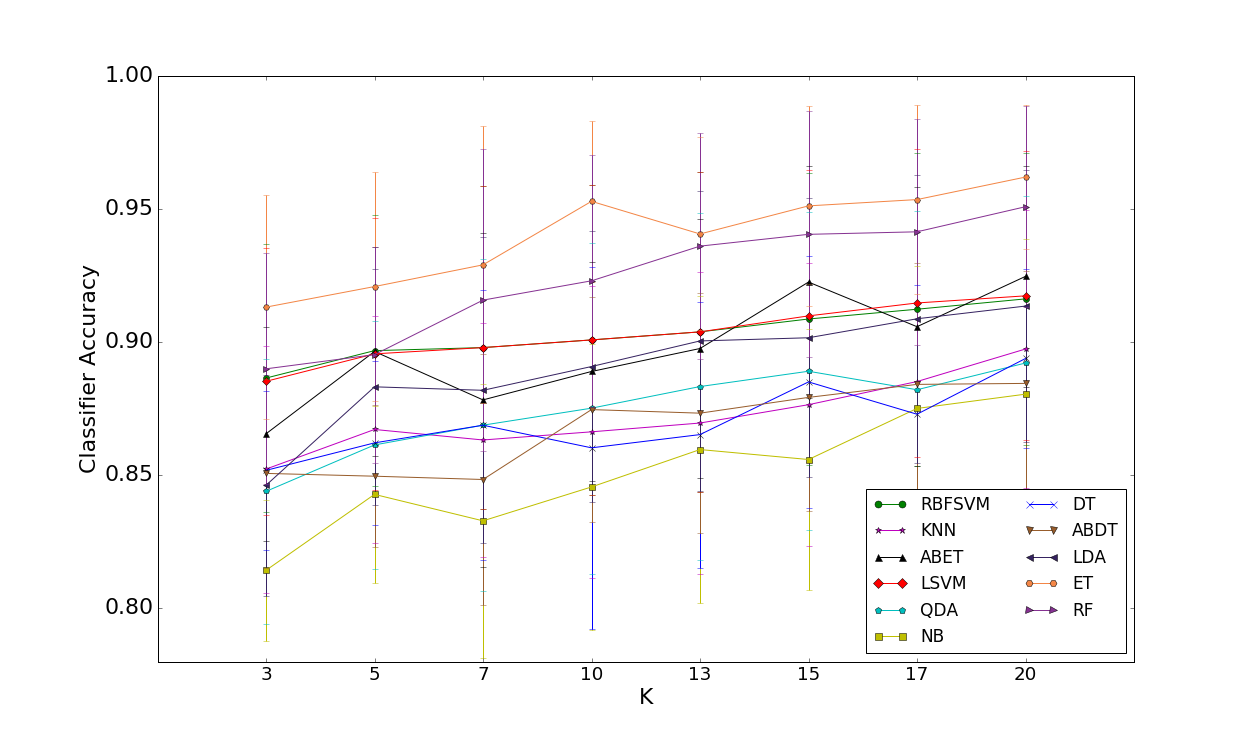
\includegraphics[]{figs/kfold}
}
\end{figure}
}
\end{frame}



\begin{frame}
\frametitle{Experiment 2 - Performance against unknown users}

\textbf{TARGET}

What is
\begin{itemize}
\item the performance for \textbf{new} / \textbf{unknown} users?
\item the \textbf{minimum} number of \textbf{users} that can be used for \textbf{training} and get an adequate classifier?
\item the effect of \textbf{``bad users''}?
\end{itemize}

\textbf{METHOD}

\begin{itemize}
\item Split the data per user
\item Use a varying number of users for training and the rest for testing
\end{itemize}

\end{frame}


\begin{frame}
\frametitle{Experiment 2 - Results per user ($F1$ score)}
\begin{table}[ht!]
\centering
\resizebox{\columnwidth}{!}{%

\begin{tabular}{l|>{\columncolor[gray]{0.9}}ccccccccccc}
\toprule
             & User 1 & User 2 & User 3 & User 4 & User 5 & User 6 & User 7 & User 8 & User 9 & User 10 & Mean w/o User 1 \\ 
\midrule
LH-SwipeDown &    0.76    &   0.83     &  1.00      &   0.82     &   1.00     &   0.80   &    1.00    &   1.00     &  1.00      &   0.96  & \textbf{0.934}    \\
LH-SwipeIn   &    0.38    &   0.92     &  0.84      &   1.00     &   1.00     &   0.92   &    1.00    &   1.00     &  1.00      &   1.00  & \textbf{0.964}    \\
LH-SwipeOut  &    0.61    &   0.93     &  0.86      &   1.00     &   1.00     &   0.89   &    1.00    &   1.00     &  0.97      &   1.00  & \textbf{0.961}    \\
LH-SwipeUp   &    0.69    &   0.90     &  1.00      &   0.84     &   1.00     &   0.83   &    1.00    &   1.00     &  0.97      &   0.96  & \textbf{0.944}    \\
RH-SwipeDown &    0.78    &   1.00     &  0.95      &    -       &   1.00     &   1.00   &    0.92    &   1.00     &  0.87      &   1.00  & \textbf{0.968}    \\
RH-SwipeIn   &    0.64    &   1.00     &  0.67      &    -       &   1.00     &   1.00   &    1.00    &   1.00     &  0.89      &   0.96  & \textbf{0.940}    \\
RH-SwipeOut  &    0.61    &   1.00     &  0.80      &    -       &   1.00     &   1.00   &    0.95    &   1.00     &  1.00      &   0.95  & \textbf{0.963}    \\
RH-SwipeUp   &    0.40    &   1.00     &  0.95      &    -       &   1.00     &   1.00   &    1.00    &   1.00     &  0.96      &   1.00  & \textbf{0.989}    \\
Average      &    \textbf{0.62}    &   \textbf{0.94}     &  \textbf{0.88}      &   \textbf{0.92}     &   \textbf{1.00}     &   \textbf{0.92}     &    \textbf{0.99}    &   \textbf{1.00}   &  \textbf{0.96}      &   \textbf{0.97}     \\
\bottomrule
\end{tabular}
}
\end{table}

\end{frame}


\begin{frame}
\frametitle{Experiment 2 - Results}
\Wider[5em]{
\begin{figure}[!htb]
\centering
\resizebox{\columnwidth}{!}{
	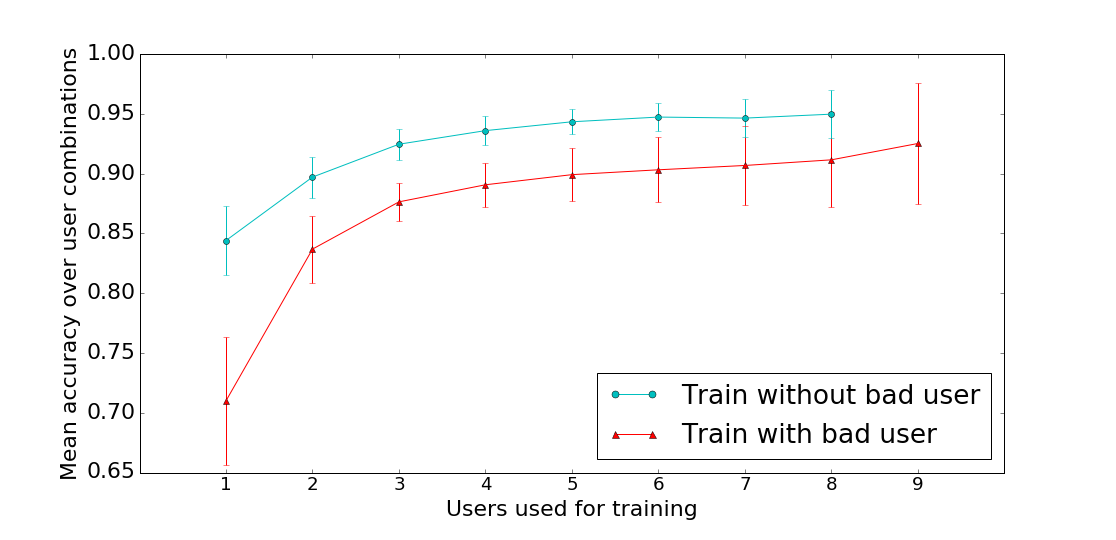
\includegraphics[]{figs/train_with_X_users}
}
\end{figure}
}
\end{frame}

\begin{frame}
\frametitle{Experiment 3 - Benchmarks}
\textbf{TARGET}
\begin{itemize}
\item Test the prediction time in different architectures
\end{itemize}

\textbf{METHOD}

Construct a custom benchmark where:
\begin{itemize}
\item \textbf{Split} the data \textbf{randomly} in train/test sets ($80$/$20$ split)
\item Classify every sample in the test data \textbf{$1000$ times}
\item Calculate the \textbf{average prediction time} for each classifier
\item Evaluate in different \textbf{architectures}
\end{itemize}

\end{frame}


\begin{frame}
\frametitle{Experiment 3 - Results}
\Wider[5em]{

\begin{figure}[!htb]
\centering
\resizebox{\columnwidth}{!}{
	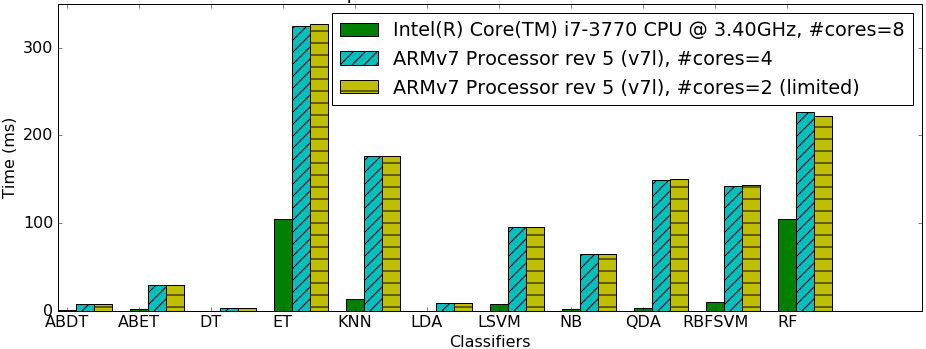
\includegraphics[]{figs/benchmark-times}
}
\end{figure}
}
\end{frame}
